\chapter{Risk Measures}
\label{var-and-credit-risk}

In quantitative finance arguably one of the most important challenge is the financial risk measurement and assessment.
The majority of the financial engineer’s task is connected to this field.
%Risk Measurement for a financial institution is very data intense and computational expensive process. Using the adequate, state of the art technologies is key to keep up with the speed of the financial market innovation, and to be able to meet the regulatory requirements.

There is a wide range of risk measures that spread through the Market: volatility ($\sigma$), Value at Risk ($VaR$), Expected Shortfall ($ES$), Conditional Value at Risk ($CVaR$) (in case of continuous distributions same as $ES$, Average Drawdown, Maximum Drawdown, $\ldots$

In the first Section of this Chapter we will concentrate specifically on two of them: $VaR$ and $ES$.

\section{VaR and Expected Shortfall}
\label{value-at-risk}

\emph{Value-at-risk} ($VaR$) is defined as the loss level that will not be exceeded with a certain confidence level during a certain period of time.
\begin{equation}
VaR_{\alpha}(X) = -F^{-1}_X(\alpha)
\label{eq:var}
\end{equation}
Mathematically it is the loss corresponding to the $(100-X)\textrm{th}$ percentile of the portfolio returns over the next $N$ days (e.g. in Figure~\ref{fig:var_loss} the graphical representation of the VaR, with $N=1$ and $X=95$, is shown; in the example a normal distribution for the changes in value is assumed). By definition it is a function of two parameters: the time horizon (i.e. $N$ days usually set to 1) and the confidence level (usually 95\%), see Fig.~\ref{fig:var_loss}. 

\begin{figure}[htb]
\centering
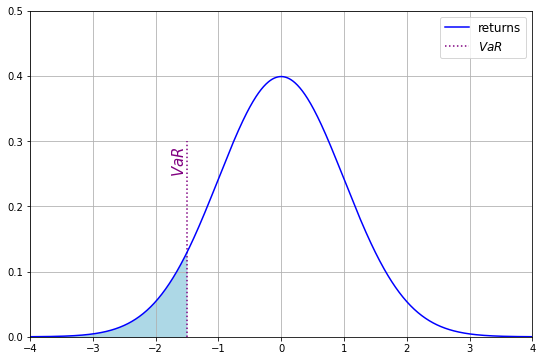
\includegraphics[width=0.6\linewidth]{figures/95_var}
\caption{Example of $VaR$ on the distribution of changes in value.}
\label{fig:var_loss}
\end{figure}

For example, if a bank's 10-day 99\% $VaR$ is 3 million USD, there is considered to be only a 1\% chance that losses will exceed 3 million USD in 10 days. One problem with $VaR$ is that, when used in an attempt to limit the risks taken by a trader, it can lead to undesirable results. Suppose a bank tells a trader that the one-day 99\% $VaR$ of the trader's portfolio must be kept less than 10 million USD. There is a danger that the trader will construct a portfolio where there is a 99\% chance that the daily loss is less than 10 million USD and a 1\% chance that it is 500 million USD. The trader is satisfying the risk limits imposed by the bank, but is clearly taking unacceptable risks. 
The problem is summarized in Figure~\ref{fig:var_vs_badvar}. It shows the probability distribution for the gain or loss on a portfolio over a specified period of time. Both portfolios have the same $VaR$. However, the portfolio on the right is much riskier than the portfolio on the left because potential losses are much larger. 

\begin{figure}[htb]
\centering
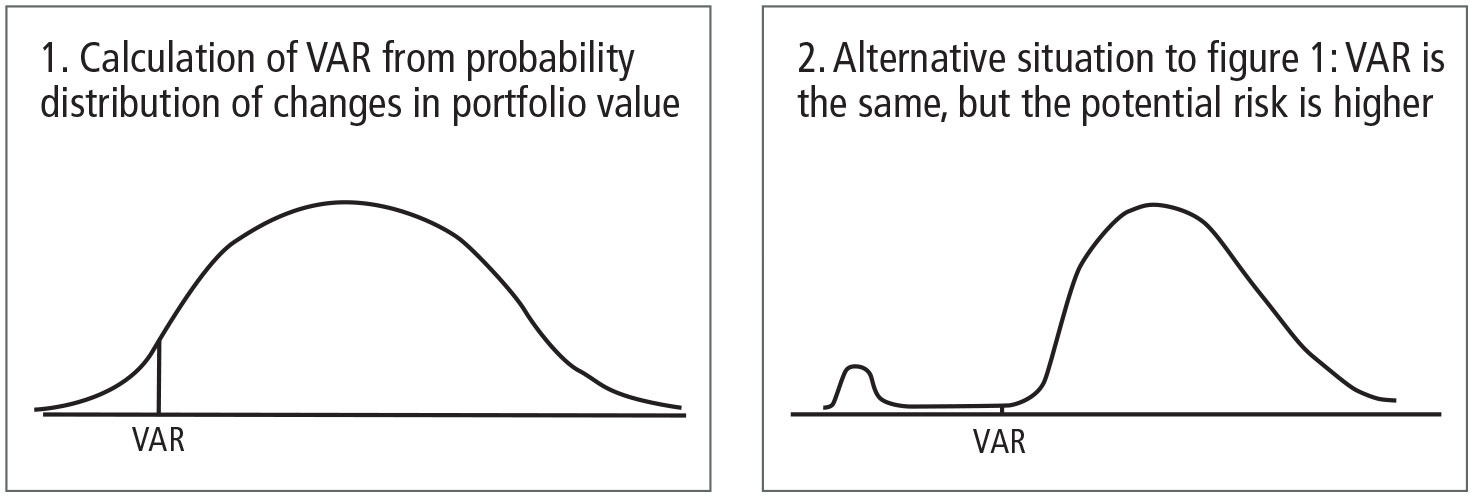
\includegraphics[width=0.8\linewidth]{figures/var_badvar}
\caption{Probability distribution for the gain or loss on a portfolio over a specified period of time. Both portfolios have the same $VaR$. However, the portfolio on the right is much riskier than the portfolio on the left because potential losses are much larger.}
\label{fig:var_vs_badvar}
\end{figure}

A measure that produces better incentives for traders than $VaR$ is \emph{expected shortfall} ($ES$). This is also sometimes referred to as conditional $VaR$. Where $VaR$ asks the question 'how bad can things get?', expected shortfall asks 'if things do get bad, what is our expected loss?'. It is the expected loss during an N-day period, conditional that the loss is greater than the $X^{th}$ percentile of the loss distribution
\begin{equation}
ES_{\alpha}(X) = \frac{1}{\alpha}\int_0^\alpha VaR_p(X) dp
\label{eq:es}
\end{equation}

For example, with $X = 99$ and $N = 10$, the expected shortfall is the average amount that is lost over a 10-day period, assuming that the loss is greater than the $99^{th}$ percentile of the loss distribution.  Clearly, the expected shortfall is much higher in Figure~\ref{fig:var_vs_badvar} (right) than (left). 

Expected shortfall is the negative of the expected value of the tail beyond the $VaR$, hence it is always a larger number than the corresponding $VaR$, see Figure~\ref{fig:es_loss}.

\begin{figure}[htb]
\centering
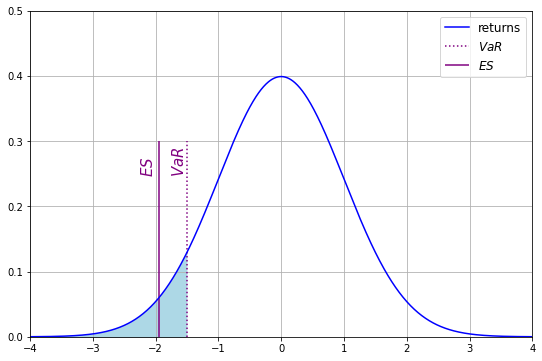
\includegraphics[width=0.6\linewidth]{figures/es}
\caption{Example of 95\% VaR on the distribution of changes in value.}
\label{fig:es_loss}
\end{figure}

Regulators make extensive use of $VaR$ and its importance as a risk measure is therefore unlikely to diminish. However, expected shortfall has a number of advantages over $VaR$, and this has led many financial institutions to use it as a risk measure internally. 

\section{How to Compute Risk Measures}
\label{how-to-estimate-the-var}

Throughout this Chapter, the historical series of Apple (AAPL) and Netflix (NFLX) stocks are used also it is assumed to have a portfolio made of \textbf{60\% of AAPL and 40\% NFLX stocks}. The dataset is available in \href{https://raw.githubusercontent.com/matteosan1/finance_course/master/input_files/historical_data.csv}{historical\_data.csv} as in the following code.

\subsection{Parametric VaR, ES}

From the historical series of the closing prices of the assets in our portfolio it can be extracted the relevant parameters of the return distribution assuming they are normal distributed.
Once the dataframe has been created the portfolio values are calculated. Then the returns are computed using \texttt{pct\_change()} method (notice that the first entry of the dataset will be \texttt{NaN} so it needs to be removed).
Finally the $\mu$ and $\sigma$ estimates are determined.

\begin{ipython}
import pandas as pd
from scipy.stats import norm
import numpy as np

df = pd.read_csv("historical_data.csv", index_col='Date')
df['P'] = df['aapl']*0.6 + df['nflx']*0.4
df = df.pct_change()
df.dropna(inplace=True)

mu = df.mean() 
sigma = df.std()

print (mu)
print (sigma)
\end{ipython}
\begin{ioutput}
0.0016446726848228527
0.020366555562177088
\end{ioutput}
\noindent
\begin{finmarkets}
The \texttt{finmarkets} module has two function to compute $VaR$ and $ES$ in the continuous case.
Since the functional form of the returns has been determined independently we can apply directly the definitions of  Eqs.~\ref{eq:var} and~\ref{eq:es}. 
For details about how to perform the integral in Eq.~\ref{eq:es} refer to Section~\ref{sec:integration}.
\end{finmarkets}

\begin{ipython}
import numpy as np
from scipy.integrate import quad

def var_continuous(f, alpha=0.95):
    return -f.ppf(1-alpha)

def es_continuous(f, alpha=0.95):
  def integrand(x, f):
    return f.ppf(x)

  alpha = 1-alpha
  I = quad(integrand, 0, alpha, args=(f,))
  return -1/alpha*I[0]
    
f = norm(mu['P'], sigma['P'])
print (f"1d-95% VaR: {var_continuous(f, 0.95):.4}")
\end{ipython}
\begin{ioutput}
1d-95% VaR: 0.03186
1d-95% ES: 0.040366
\end{ioutput}

Many influential theories in finance assume the normality of stock returns: portfolio theory and CAPM (where normality of returns implies that
only the mean and variance are relevant for portfolio optimization), option pricing theory (Black and Scholes model assumes (log-)returns follow a Brownian motion, i.e., are normally distributed over any given time interval).
Unfortunately normality is not a realistic assumption as can be seen by performing a Gaussian fit to the return distribution.

\begin{figure}[htb]
\centering
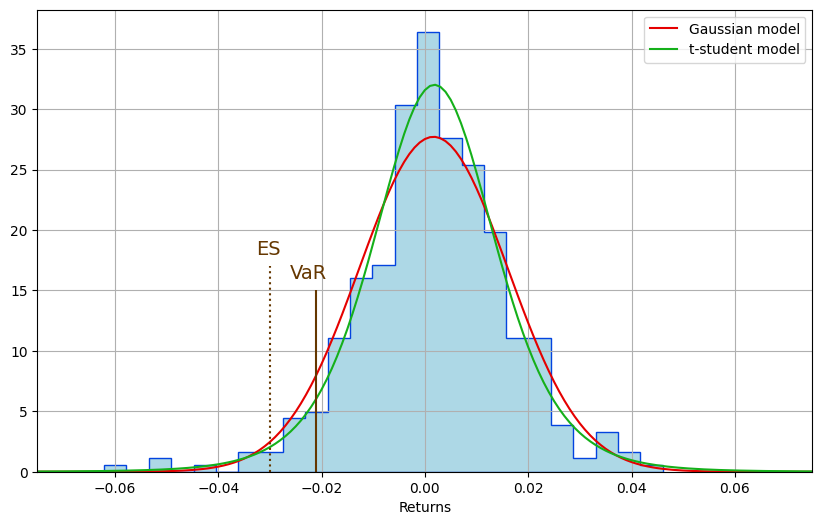
\includegraphics[width=0.6\textwidth]{figures/parametric_var}
\caption{Return distribution obtained from the historical data used in the example. The red line shows the 99\% VaR. The distribution has also been fitted with a Gaussian and a t-student and the results are shown with the dashed lines.}
\label{fig:paramtric_var}
\end{figure}

Dashed lines in Figure~\ref{fig:paramtric_var} shows the resulting fit which clearly doesn't follow well the underlying distribution, so returns are \textbf{not} normally distributed. Much better results can be obtained with a t-student distribution. The fit is shown by green line in Fig.~\ref{fig:paramtric_var}. A better model results in a more precise estimate of $VaR$ and $ES$. The calculation is similar to the previous one, it is enough to pass to the two functions the fitted model.

\begin{ipython}
from scipy.stats import t

f2 = t.fit(df['P'])
model = t(*f2)

print (f"1d-95% VaR: {var_continuous(model, 0.95):.4}")
print (f"1d-95% ES: {es_continuous(model, 0.95):f}")
\end{ipython}
\begin{ioutput}
1d-95% VaR: 0.02803
1d-95% ES: 0.047245
\end{ioutput}

\subsection{Historical Simulation}
\label{historical-simulation}

It is possible to avoid any assumption on the return distribution, by random sampling on the historical returns directly. The parameter estimation is not required in this case, but clearly such kind of simulation heavily relies on the assumption that past behaviors are indicative of what might happen in the future. That's why it is important that out historical series was as large as possible otherwise our results will be affected by lack of statistics. 

\begin{finmarkets}
The \texttt{finmarkets} module has also two functions to compute $VaR$ and $ES$ for the discrete case. 
They rely on the sampling from the original historical series which has been implemented in a separated utility function. The fastest way to generate random sample of historical returns is to assign an integer for each observation, and, using a random sampling algorithm, we can generate the set of simulated returns. Then the risk measures are calculated as percentiles of the the generated distributions. Notice that \texttt{numpy.random.choice} is equivalent to \texttt{random.sample} that we have already used before.
\end{finmarkets}

\begin{ipython}
from numpy.random import choice
from numpy import percentile

def generate_returns(df, N=100000):
    data = df.reset_index()
    return data.loc[choice(range(len(data), N)]
    returns = df2['P'].loc[return_indexes]

def var_discrete(df, alpha=0.95):
    alpha = 1-alpha
    return -percentile(df, alpha*100)
    
def es_discrete(df, alpha=0.95):
    alpha = 1-alpha
    var = percentile(df, alpha*100)	
    return -df[df<=var].mean()
    
returns = generate_returns(df, 10000)
print (f"1d-95% VaR (discrete): {var_discrete(returns['P'], 0.95):.4f}")
print (f"1d-95% ES (discrete): {es_continuous(model, 0.95):.4f}")
\end{ipython}
\begin{ioutput}
1d-95% VaR (discrete): 0.02661
1d-95% ES (discrete): 0.04328
\end{ioutput}

Figure~\ref{fig:historical_var} shows the results. Notice again that the generated return distributions suffers from the same limitation of the original historical series (e.g. missing data in specific regions).

\begin{figure}[htb]
\centering
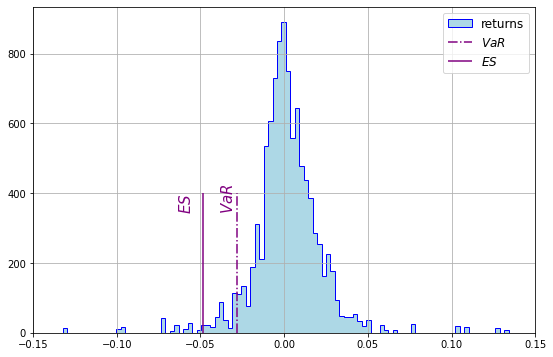
\includegraphics[width=0.6\textwidth]{figures/historical_var}
\caption{Distribution of the return random sampling. The corresponding $VaR$ and $ES$ are also shown.}
\label{fig:historical_var}
\end{figure}

\subsection{Stress and Back Testing}
\label{stress-testing-and-back-testing}

In addition to calculating a portfolio risk measure, it is generally useful to check how the portfolio would behave under the most extreme market moves seen in the last years.

This kind of test is called \emph{stress test} and it is done by extracting from the historical series particular days with exceptionally large variation of the market variables.
The idea is to take into account extreme events that can happen more frequently in reality than in a simulation (where usually Gaussian tails are assumed). 

Another important check that could be done is the \emph{back testing} which consists of assessing how well the $VaR$ (or $ES$) estimate would have performed in the past. Basically it has to be tested how often the daily loss exceeded the N-days $X\%$ $VaR$ just computed. If it happens on about $(100-X)\%$ of the times we can be confident that our estimate is correct. Clearly back-testing makes sense only if $VaR$ has been estimated on an independent historical sample with respect to that used in the risk measure calculations.

\begin{ipython}
print ((df['P'] < -v1).sum()/len(df))
\end{ipython}
\begin{ioutput}
0.044131455399061034
\end{ioutput}

\section{Credit VaR}
\label{credit-var-cr-var}

%exposure at any given future time is the
%larger between zero and the market value of the portfolio of derivative
%positions with a counterparty that would be lost if the counterparty
%were to default with zero recovery at that time.

\emph{Credit VaR} is defined in the usual way other risk measures are (i.e. as percentile of a loss distribution). In this case we are concerned with the default risk associated to one or multiple counter-parties in a specific portfolio instead with to the market risk.

To derive the loss distribution we need to consider the exposure $\textrm{EE}(\tau)$ defined as the sum of the discounted cash flows at the default date $\tau$. The corresponding loss is then given by

\begin{equation}
L_{\tau} = (1 - R) \cdot \textrm{EE}(\tau)
\end{equation}
where $L$ is non-zero only in scenarios of early counter-party default. 

Given the above definitions we can express the Credit VaR as the (100-X)-quantile of $L_{\tau}$. With respect to the Value at Risk, the time horizon is usually set to one year and the percentile to $99.9^{th}$, so it returns the loss that is exceeded only in 1 case out of 1000. 

Note that in this case quantile has to be computed on the "positive" tail of the loss distribution, because $L$ represents the loss value (i.e. it is a positive quantity).

Credit VaR is actually either the difference of the percentile from the mean, or the percentile itself. There is more than one possible definition, anyway we  will use the latter.

%Consider your portfolio has a call option on equity with a final maturity of two years. To get the Credit-Var, roughly, you simulate the underlying equity up to one year, and obtain a number of scenarios for the underlying equity in one year. Also, you need to simulate the default scenarios up to one year, to know in each scenario whether the counter-parties have defaulted or not. 
%
%And then in each scenario at one year, if the counter-party
%has defaulted there will be a recovery value and all else will be lost.
%Otherwise, we price the call option over the remaining year using for
%example a Black Scholes formula. But this price is like taking the
%expected value of the call option payoff in two years, conditional on
%each scenario for the underlying equity in one year. Because this is
%pricing, this expected value will be taken under the pricing measure Q,
%not P. This gives the Black Scholes formula if the underlying equity
%follows a geometric brownian motion under Q.

\subsection{Credit VaR and MC Simulation}
\label{sec:credit-var-sim}
Credit VaR can be calculated through a simulation of the evolution of a portfolio up to the risk horizon; the simulation must of course include possible defaults of the counter-parties. 
In each experiment the portfolio is priced obtaining a number of scenarios to draw the loss distribution. It is then straightforward to derive the Credit VaR.

Consider, for example, a portfolio of five fixed coupon bonds (0.1) each one with the same default probability (a Poisson process with $\lambda=0.5$) and the same face value (100 EUR). The recovery rate in case of default is $R=40\%$ and the discount curve is the one stored in \href{https://github.com/matteosan1/finance_course/raw/master/input_files/discount_factors_2022-10-05.xlsx}{discount\_curve.xlsx}.

In order to better simulate the evolution of the portfolio a helper function \texttt{Bond} is implemented: it is just able to compute the bond NPV at a given date. Also a set of default times has been calculated using \texttt{PoissonProcess} distribution.
Notice that in this simple example there is no need to run multiple scenarios since any market parameters of the portfolio is changing and no evolution is required (e.g. interest rate is fixed).
 
\begin{ipython}
from finmarkets import generate_dates, maturity_from_str

class Bond:
    def __init__(self, face_value, start_date, tenor, maturity):
        self.FV = face_value
        self.tau = maturity_from_str(tenor, "y")
        self.payment_dates = generate_dates(start_date, maturity, tenor)

    def npv(self, d, dc, fc):
        val = 0
        for i in range(1, len(self.payment_dates)):
            C = fc.forward_rate(self.payment_dates[i-1], self.payment_dates[i])
            if self.payment_dates[i-1] <= d < self.payment_dates[i]:
                rateo = (self.payment_dates[i] - d).days/
                (self.payment_dates[i] - self.payment_dates[i-1]).days
                val += C*rateo*self.tau*dc.df(d)
            elif self.payment_dates[i] > d:
                val += C*self.tau*dc.df(self.payment_dates[i])
                val += dc.df(self.payment_dates[-1])
        return self.FV*val
\end{ipython}
\begin{ipython}
import pandas as pd
import numpy as np
from datetime import date
from dateutil.relativedelta import relativedelta
from finmarkets import DiscountCurve, CreditCurve, ForwardRateCurve
from finmarkets import PoissonProcess, generate_dates
    
start_date = date.today()
df = pd.read_excel("discount_curve.xlsx")
pillars = [start_date + relativedelta(months=i) for i in df['months']]
dc = DiscountCurve(pillars, df['dfs'])

bonds = []
maturity = "2y"

fc_dates = generate_dates(start_date, maturity, "1y")
rates = [0.1 for _ in range(len(fc_dates))]
fc = ForwardRateCurve(start_date, fc_dates, rates)

for i in range(len(coupons)):
    bonds.append(Bond(100, start_date, coupons[i], 1, maturity))

np.random.seed(1)
N = 100000
R = 0.4
horizon = 1

Q = PoissonProcess(l=0.5)
cov = np.ones(shape=(len(bonds), len(bonds)))*rho
np.fill_diagonal(cov, 1)
g = GaussianCopula(len(bonds), cov)
taus = Q.ppf(g.sample(N))

L = []
for n in range(N):
    EE = 0
    for i, b in enumerate(bonds):
        if taus[n, i] <= horizon:
            d = start_date + relativedelta(days=365*taus[n, i])
            EE += b.npv(dc, d)
    if EE != 0:
        L.append((1-R)*EE)
  
print (np.percentile(L, [95.0]))
\end{ipython}
\begin{ioutput}
338.0718924883006
\end{ioutput}
\noindent
Figure~\ref{fig:credit_var} shows the loss distribution of the portfolio. Each peak corresponds to scenarios where there is an increasing number of defaults and is located roughly at multiple of 60 since each bond value is around 100 which gives a loss of that size (i.e. $1-R$ with $R\simeq$40\%). 

\begin{figure}[htb]
\centering
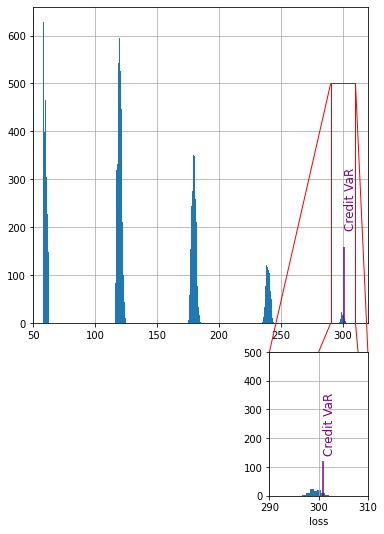
\includegraphics[width=0.5\textwidth]{figures/credit_var}
\caption{Distribution of losses in a portfolio made of five fixed coupon bonds. In the zoom the tail of the plot is shown to highlight the Credit VaR value.}
\label{fig:credit_var}
\end{figure}

\subsection{Credit VaR and One Factor Copula Model}
Consider a portfolio made of similar assets. As an approximation assume that the probability of default is the same for each counter-party and that the correlation between each pair is the same and equal to $\rho$. Under these assumption the One Factor Copula model can be used to describe the default correlations (see Eq.~\ref{eq:gaussian_one_factor_copula}

\begin{equation}
\mathcal{Q}_M(T) = \Phi\Big(\cfrac{\Phi^{-1}[Q(T)]-M\sqrt{\rho}}{\sqrt{1-\rho}}\Big)
\label{eq:conditional_default_prob}
\end{equation}
where $\Phi$ is the cumulative distribution function of the standard normal.

Since there are $n$ counter-parties with the same default probability $\mathcal{Q}_M(T)$ the percentage of defaults at time $T$ is $\mathcal{Q}_M$ itself ($\textrm{\% of defaults} = \textrm{n\_defaults}/n = n\cdot \mathcal{Q}_M/n$). Hence Eq.~\ref{eq:conditional_default_prob} gives the percentage of defaults by time $T$ given $M$. 

Since $M$ is distributed according to a standard Gaussian we can be $X\%$ certain that its value will be \emph{greater} than $\hat{m} = \Phi^{-1}(1-X)=-\Phi^{-1}(X)$, where the equality holds due to the symmetry of the Gaussian distribution (see Figure~\ref{fig:certain_for_X}).

\begin{figure}[htb]
\centering
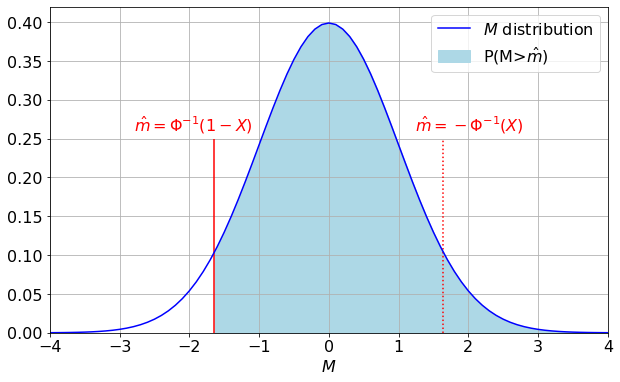
\includegraphics[width=0.7\textwidth]{figures/certain_for_X}
\caption{$X\%$ probability to get an higher value a threshold for a normally distributed random variable.}
\label{fig:certain_for_X}
\end{figure} 

Once the time $T$ has been chosen the only random variable appearing in the conditional default probability expression of Eq.~\ref{eq:conditional_default_prob} is $M$, therefore we can be $X\%$ certain that the percentage of defaults over $T$ years on a large portfolio will be \textbf{less} than $V(X,T)$ where

\begin{equation*}
V(X,T)= \Phi\Big(\cfrac{\Phi^{-1}[Q(T)]-\hat{m}\sqrt{\rho}}{\sqrt{1-\rho}}\Big) = \Phi\Big(\cfrac{\Phi^{-1}[Q(T)]+\Phi^{-1}(X)\sqrt{\rho}}{\sqrt{1-\rho}}\Big)
\end{equation*}

When the confidence level is $X\%$ and the time horizon is $T$, a rough estimate of the Credit VaR is therefore $P(1-R)V(X,T)$, where $P$ is the portfolio size and $R$ is the recovery rate.

Suppose that a bank has a total of \euro{100} million of retail exposures. The 1-year probability of default averages to 2\% and the recovery rate averages to 60\%. The copula correlation parameter is estimated as 0.1.

\begin{ipython}
from scipy.stats import norm
from math import sqrt

X = 0.999
rho = 0.1
R = 0.6
Q = 0.02
exposure = 100e6
num = norm.ppf(Q) + sqrt(rho)*norm.ppf(X)
den = sqrt(1-rho)
V = norm.cdf(num/den)
cr_var = exposure*V*(1-R)

print (f"Cr-VaR: {round(cr_var, -4):.0f}")
\end{ipython}
\begin{ioutput}
Cr-VaR: 5130000
\end{ioutput}
\noindent
The 1-year 99.9\% Credit VaR is therefore \euro{5.13} million.

\subsection{CreditMetrics}
Another popular approach to estimate Credit VaR is \emph{CreditMetrics}. It involves computing a probability distribution of credit losses by carrying out Monte Carlo simulations of the counter-party credit rating changes.

Imagine we would like to determine the probability distribution of losses over 1-year period. On each simulation, we are going to determine the credit rating of each counter-party using the estimated probability of migration between one rate to another (or to default). Since the portfolio value depends on its asset ratings we can determine the eventual losses. 

As an example consider Table~\ref{tab:credit_ratings} which shows the percentage probability of a bond moving from one category to another during a 1-year period.

\begin{table}[htb]
\centering
\begin{tabular}{|l|c|c|c|c|c|c|c|c|}
\hline
Initial rating & AAA & AA & A & BBB & BB & B & CCC & default \\
\hline
\hline
AAA & 90.81 & 8.33 & 0.68 & 0.06 & 0.08 & 0.02 & 0.01& 0.01 \\ 
\hline
AA & 0.70 & 90.65 & 7.79 & 0.64 & 0.06 & 0.13 & 0.02 & 0.01 \\ 
\hline
A & 0.09 & 2.27 & 91.05 & 5.52 & 0.74 & 0.26 & 0.01 & 0.06 \\ 
\hline
BBB & 0.02 & 0.33 & 5.95 & 85.93 & 5.30 & 1.17 & 1.12 & 0.18 \\
\hline
BB & 0.03 & 0.14 & 0.67 & 7.73 & 80.53 & 8.84 & 1.00 & 1.06 \\
\hline
B & 0.01 & 0.11 & 0.24 & 0.43 & 6.48 & 83.46 & 4.07 & 5.20 \\
\hline
CCC & 0.21 & 0 & 0.22 & 1.30 & 2.38 & 11.24 & 64.86 & 19.79 \\		
\hline
\end{tabular}
\caption{Example of table with transition probabilities (in percent) between different credit rating categories.}
\label{tab:credit_ratings}
\end{table}

For a correct implementation of this technique credit rate changes cannot be assumed independent, hence a copula approach could be implemented.
Another possibility is the application of Markov chains~\ref{sec:markov_chain}, with the transition matrix which can be deduced by the numbers in Table~\ref{tab:credit_ratings}.

In fact the main difficulty in this application is precisely the determination of the transition matrix. These probabilities could be estimated by analyzing historical data from credit rating agencies, such as Standard\&Poor, Moody's and Fitch. But this could lead to unreliable numbers in case the future does not develop as smoothly as the past. It can therefore be more reliable to base the estimates on a combination of empirical data and more subjective, qualitative data such as opinions from experts. This is because the market view is a mixture of beliefs determined by both historical ratings and a more extreme view of the ratings. 

Another problem with deciding the transition matrix is that maybe it is not appropriate to use a \emph{homogeneous} Markov chain to model credit risk over time. In this kind of chain the transition matrix is considered constant, but it is clearly a crude approximation of reality which doesn't capture the time-varying behavior of the default risk. A non-homogeneous model could be more realistic, but on the other hand more complicated to use. 

\section{Credit Valuation Adjustment}
\label{credit-valuation-adjustment}

Suppose you have a portfolio of derivatives. If a counter-party defaults and the present value of the portfolio at default is positive to the surviving party (you), then the actual gain is only given by the recovery fraction of the value. If however the present value is negative to you, you have to pay it in full to the liquidators of the defaulted entity.

This behavior creates an asymmetry which can be corrected by changing the definition of the deal value as the value without counter-party risk minus a positive adjustment, called \emph{Credit Valuation Adjustment} (CVA).

The CVA can be expressed in the following way:

\begin{equation}
\text{CVA} = (1-R) \int_0^T D(t) \cdot \textrm{EE}(t) dQ(t)
\label{eq:cva}
\end{equation}
where $T$ is the latest maturity in the portfolio, $D$ is the discount factor, EE is the expected exposure or $\mathbb{E}[\max(0, NPV_{portfolio})]$, and $dQ$ is the probability of default between $t$ and $t+dt$.

For an easier computation it is natural to discretize the above integral and use a time grid going from 0 to the portfolio maturity:

\begin{equation}
\text{CVA} = (1-R) \sum_i^n D(t_i) \cdot \mathrm{EE}(t_i) Q(t_{i-1}, t_i)
\label{eq:cva_discrete}
\end{equation}

It is important to note the difference between Credit VaR and CVA. While the former measures the risk of losses faced due to the possible default of some counter-party, the latter measures the pricing component of this risk, i.e. the price adjustment of a contract due to this risk.

\subsection{Debit Valuation Adjustment}

The adjustment seen from the point of view of our counter-party is positive, and is called Debit Valuation Adjustment, DVA. It is positive because the early default of the client itself would imply a discount on its payment obligations, and this means a gain. So the client marks an adjustment over the risk free price by adding the positive amount called DVA. 

When both parties have non-null default probabilities, they consistently include both defaults into the valuation. So they will mark a positive CVA to be subtracted and a positive DVA to be added to the default risk free price of the deal. The CVA of one party will be the DVA of the other one and vice versa.

\begin{equation*}
\textrm{price}=\textrm{default risk free price + DVA - CVA}
\end{equation*}
Now, since
\begin{equation*}
\begin{gathered}
\textrm{default risk free price(A)} = - \textrm{default risk free price(A)} \\
\textrm{DVA(A)} = \textrm{CVA(B)} \\
\textrm{DVA(B)} = \textrm{CVA(A)} 
\end{gathered}
\end{equation*}
we get that eventually
\begin{equation*}
\textrm{price(A)} = -\textrm{price(B)}
\end{equation*}
so that both parties agree on the price, or, we could say, there is money conservation.

\subsection{CVA Computation}

The computation of the CVA is carried on with Monte Carlo simulation. 
First calculate the portfolio value at each time point for each MC scenario. Then estimate the CVA using either Eq.~\ref{eq:cva} or its discrete form in Eq.~\ref{eq:cva_discrete}. Finally average the CVA of all the scenarios to get its value.

In case of zero coupon bonds the computation of the CVA can be further simplified. Indeed in this case the investor exposure is equal to the bond face value, so it is enough to loop through each day from the pricing date to the bond maturity and compute the CVA using Eq.~\ref{eq:cva_discrete}.

Imagine a 3-years coupon bond with a face value of $FV=$~\euro{100}. The bond issuer has the following default probabilities 10\%, 20\% and 30\% for 1, 2 and 3 years respectively and the recovery rate is 40\%. The discount factors can be determined from \href{https://github.com/matteosan1/finance_course/raw/master/input_files/discount_factors_2022-10-05.xlsx}{discount\_curve.xlsx}.
In order to simulate the interest rate evolution the Vasicek model~\ref{vasicek-model} has been used with parameters: $\kappa=-0.137$, $\theta=-0.00179$ and $\sigma=0.00187$. 

\begin{ipython}
import numpy as np
from datetime import date

from finmarkets import generate_dates
from finmarkets.short_rates.vasicek import VasicekModel

M = 1000
rates = []
start_date = date.today()

v = VasicekModel(-0.137, -0.00179, 0.00187)
dates = generate_dates(start_date, "3y", "3m")
for i in range(M):
    rates.append(v.r_generator(0.035, dates, i))
\end{ipython}

\begin{figure}[htb]
\centering
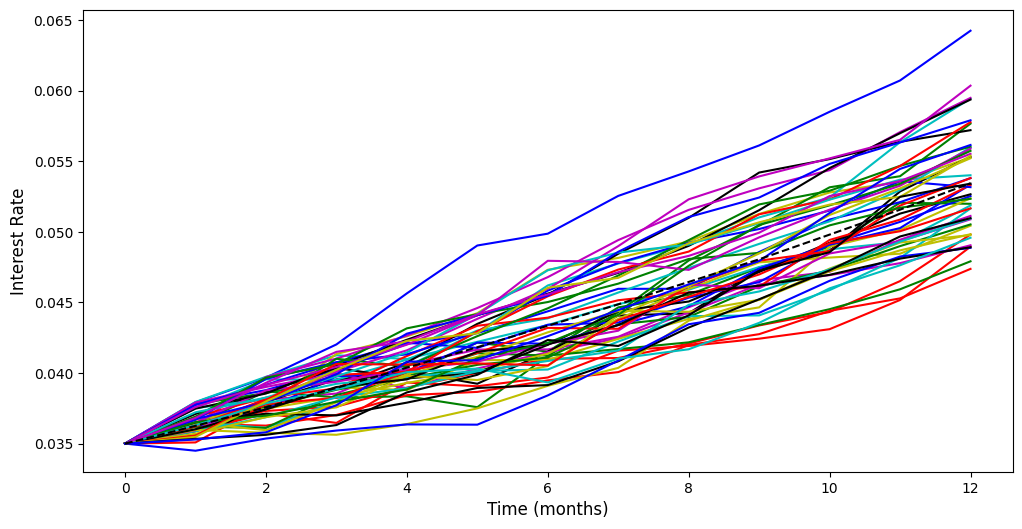
\includegraphics[width=0.7\textwidth]{figures/vasicek_simulation}
\caption{Simulation of 1000 interest rate paths with Vasicek model, only few of them are reported. The dashed line shows the average path. The spot rate is assumed to be 3.5\%.}
\label{fig:vasicek_simulation}
\end{figure} 

To calculate the CVA we need to first define a discount curve and the issuer credit curve. Then we perform a daily loop to sum up all the contributions to the CVA (averaged over the interest rate paths) and finally set the price of the bond to the default-risk-free price minus the CVA.
Notice that the code below is relying on the \texttt{Bond} class implemented in~\ref{sec:credit-var-sim}.

\begin{ipython}
import pandas as pd

from dateutil.relativedelta import relativedelta
from finmarkets import DiscountCurve, CreditCurve, ForwardRateCurve

df = pd.read_excel("discount_curve.xlsx")
pillars = [start_date + relativedelta(months=i) for i in df['months']]
dc = DiscountCurve(start_date, pillars, df['dfs'])

pillar_dates = [start_date + relativedelta(years=i) for i in range(4)]
S = [1, 0.9, 0.8, 0.7]
cc = CreditCurve(start_date, pillar_dates, S)

fc = ForwardRateCurve(start_date, fc_dates, avg)

bond = Bond(100, start_date, "3m", "3y")
PV = bond.npv(start_date, dc, fc)

R = 0.4
cva = 0
d = start_date
while d < pillar_dates[-1]:
    cvas = 0
    if d+relativedelta(months=1) > pillar_dates[-1]:
        break
    dP = cc.ndp(d)-cc.ndp(d+relativedelta(months=1))
    for i in range(M):
        fc = ForwardRateCurve(start_date, fc_dates, rates[i])
        cvas += (1-R)*max(0, bond.npv(d, dc, fc))*dP
    cva += cvas/M
    d += relativedelta(months=1)

print ("CVA: {:.2f}".format(cva))	
print (f"Adjusted Price: {PV-cva:.2f} EUR")
\end{ipython}
\begin{ioutput}
CVA: 18.28 EUR
Adjusted Price: 90.05 EUR
\end{ioutput}

\section*{Exercises}
\begin{question}
Given the historical series of three stock prices in the file \href{https://raw.githubusercontent.com/matteosan1/finance_course/master/input_files/historical.csv}{historical.csv} compute the 1-day 95\% VaR and the corresponding Expected shortfall for a portfolio consisting of 40 FOX shares, 35 ABC shares and 25 CBS shares. 

\noindent\textbf{Hint:} when simulating the historical scenarios take care of possible NaN values in the series.
\end{question}

\cprotEnv\begin{solution}
\begin{ipython}
import pandas as pd
import numpy as np

df = pd.read_csv("historical.csv", index_col='date')
w = np.array([0.4, 0.25, 0.35])

df['P'] = df[['FOX', 'CBS', 'ABC']].dot(w)
df = df.pct_change()
df.dropna(inplace=True)
print (df.head())
\end{ipython}
\begin{ioutput}
                 FOX       CBS       ABC         P
date                                              
2018-03-26  0.013858 -0.012607  0.011189  0.006395
2018-03-23 -0.030891 -0.046818 -0.010830 -0.024072
2018-03-22  0.020592  0.020093  0.011543  0.015722
2018-03-21  0.003317  0.012137  0.052941  0.031266
2018-03-20 -0.003306 -0.011991 -0.003464 -0.005276
\end{ioutput}
\begin{ipython}
from numpy.random import seed, choice
from numpy import percentile
from finmarkets import var_discrete, es_discrete
 
var = var_discrete(df, 0.95, 'P')
es = es_discrete(df, 0.95, 'P')

print (f"VaR: {var:.4f}")
print (f"ES: {es:.4f}")
\end{ipython}
\begin{ioutput}
VaR: 0.0173
ES: 0.0232
\end{ioutput}
\begin{figure}[htbp]
\centering
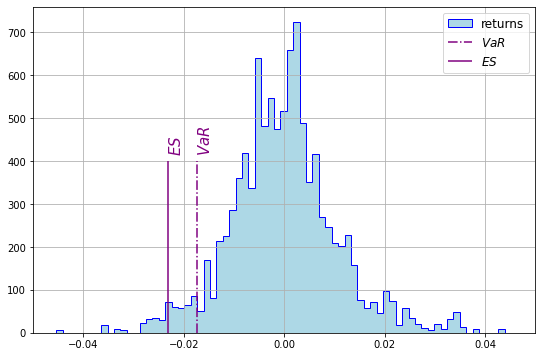
\includegraphics[width=0.7\linewidth]{figures/hist_var_ex}
\end{figure}
\end{solution}

\begin{question}
You have a 3-years call with strike 110 EUR. The underlying initial price is 105 EUR with a volatility of 0.15. The risk-free rate is 0.03 flat.
Compute the CVA of the contract assuming a recovery rate of 40\% and default probabilities for the underlying of 10\%, 20\% and 30\% for first, second and third year respectively.
\end{question}

\cprotEnv\begin{solution}
Below are shown ten realizations of the underlying price.

\begin{figure}[htbp]
\centering
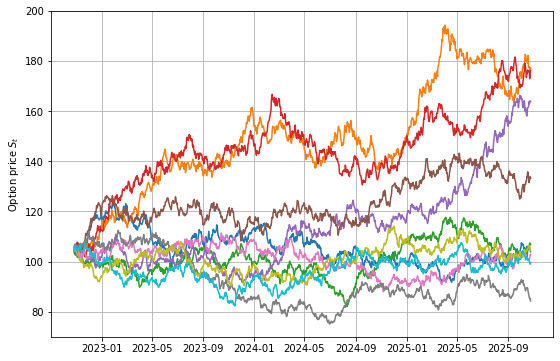
\includegraphics[width=0.7\linewidth]{figures/underlying_simulation}
\end{figure}

This implementation is not optimized in terms of speed, indeed it takes about 2 minutes to run 500 simulations.
A different approach, fully exploiting \texttt{numpy.array}s, could allow to shrink the execution time by a factor of 200.

\begin{ipython}
from datetime import date
from dateutil.relativedelta import relativedelta
from finmarkets import CreditCurve, call
from scipy.stats import norm
import numpy as np
import time

K = 110
sigma = 0.15
r = 0.03
T = 3
steps = 365*T
dt = 1/365
R = 0.4
Q = [0.9, 0.8, 0.7]
S0 = 105

obs_date = date.today()
dates = [obs_date + relativedelta(years=i+1) for i in range(T)]
cc = CreditCurve(obs_date, dates, Q)
t1 = time.time()
scenarios = 500
St = np.zeros(shape=(steps, scenarios))
St[0, :] = S0
ndps = np.zeros(shape=(steps,))
for i in range(1, steps):
    St[i, :] = St[i-1, :] * np.exp((r - 0.5 * sigma**2) * dt \
        + sigma* np.sqrt(dt) * norm.rvs(size=scenarios))
    ndps[i] = cc.ndp(obs_date+relativedelta(days=i-1)) - \
        cc.ndp(obs_date+relativedelta(days=i))

ts = [f"{t}y" for t in np.arange(T-dt, 0, -dt)]
cvas = np.zeros(shape=(steps, scenarios))
for s in range(scenarios):
    for j in range(len(ts)):
        cvas[j, s] = call(St[j, s], K, r, sigma, ts[j])*(1-R)*ndps[j]
cvas = np.sum(cvas, axis=0)
print (np.mean(cvas))
print (time.time() - t1)
\end{ipython}
\begin{ioutput}
2.464147656202549
129.0265169143676
\end{ioutput}
\end{solution}

\begin{question}
\label{ex:credit_var}
Consider a 1-years call with strike 110 EUR. The underlying initial price is 100 EUR with a volatility of 0.50. The risk-free rate is 0.03 flat. Compute the 99.9\% Credit VaR assuming a recovery rate of 40\% and default probabilities for the underlying of 30\% within next year.
\end{question}

\cprotEnv\begin{solution}

In order to increase the number of simulations the implemented code fully uses \texttt{numpy.array}.

\begin{ipython}
import numpy as np
from datetime import date
from dateutil.relativedelta import relativedelta
from finmarkets import CreditCurve
from scipy.stats import norm


K = 110
sigma = 0.50
r = 0.03
T = 1
steps = 365*T
dt = 1/365
R = 0.4
S0 = 100

obs_date = date.today()
cc = CreditCurve(obs_date, [obs_date + relativedelta(years=1)], [0.7])
scenarios = 10000
St = np.zeros(shape=(steps, scenarios))
St[0, :] = S0
ndps = np.zeros(shape=(steps,))
for i in range(1, steps):
    St[i, :] = St[i-1, :] * np.exp((r - 0.5 * sigma**2) * dt \
                                   + sigma* np.sqrt(dt) * norm.rvs(size=scenarios))
    ndps[i] = cc.ndp(obs_date+relativedelta(days=i)) - \
        cc.ndp(obs_date+relativedelta(days=i+1))

ts = [f"{t}y" for t in np.arange(T-dt, 0, -dt)]
EE = np.zeros(shape=(steps, scenarios))
for s in range(scenarios):
    EE[1:, s] = call(St[:-1, s], K, r, sigma, ts)*(1-R)*ndps[1:]
EE = np.sum(EE, axis=0)
print (f"Credit VaR: {np.percentile(EE, 99.9):.3f}")
\end{ipython}
\begin{ioutput}
Credit VaR: 26.281
\end{ioutput}

\begin{figure}[htbp]
\centering
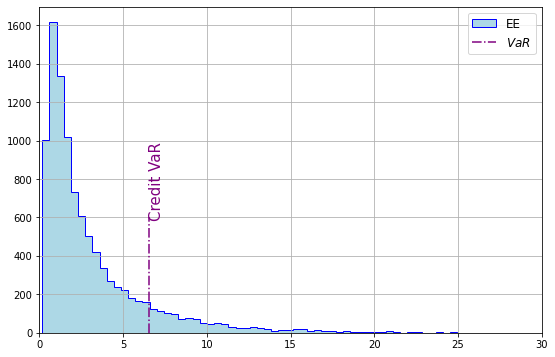
\includegraphics[width=0.7\linewidth]{figures/cr_var_ex}
\caption{Loss distribution to estimate Credit VaR measure of Ex.~\ref{ex:credit_var}.}
\end{figure}
\end{solution}







\begin{thebibliography}{9}
\bibitem{bib:var} J. C. Hull, \emph{Options, Futures and Other Derivatives, 7th Ed.}, Value at Risk (Ch. 20), Pearson Prentice Hall, 2009
\bibitem{bib:credit_var} J. C. Hull, \emph{Options, Futures and Other Derivatives, 7th Ed.}, Credit Risk (Ch. 22), Pearson Prentice Hall, 2009
\bibitem{bib:creditmetrics}RiskMetrics Group, \href{https://www.msci.com/documents/10199/93396227-d449-4229-9143-24a94dab122f}{\emph{CreditMetrics}}, J.P. Morgan \& Co., 2007, [Online]
\bibitem{bib:cva} D. Brigo, \emph{Counterparty Risk FAQ: Credit VaR, PFE, CVA, DVA, Closeout, Netting, Collateral, Re-hypothecation, WWR, Basel, Funding, CCDS and Margin Lending}, arXiv: 1111.1331, 2011
\end{thebibliography}
